% Options for packages loaded elsewhere
\PassOptionsToPackage{unicode}{hyperref}
\PassOptionsToPackage{hyphens}{url}
%
\documentclass[
  11pt,
]{article}
\usepackage{lmodern}
\usepackage{amssymb,amsmath}
\usepackage{ifxetex,ifluatex}
\ifnum 0\ifxetex 1\fi\ifluatex 1\fi=0 % if pdftex
  \usepackage[T1]{fontenc}
  \usepackage[utf8]{inputenc}
  \usepackage{textcomp} % provide euro and other symbols
\else % if luatex or xetex
  \usepackage{unicode-math}
  \defaultfontfeatures{Scale=MatchLowercase}
  \defaultfontfeatures[\rmfamily]{Ligatures=TeX,Scale=1}
\fi
% Use upquote if available, for straight quotes in verbatim environments
\IfFileExists{upquote.sty}{\usepackage{upquote}}{}
\IfFileExists{microtype.sty}{% use microtype if available
  \usepackage[]{microtype}
  \UseMicrotypeSet[protrusion]{basicmath} % disable protrusion for tt fonts
}{}
\makeatletter
\@ifundefined{KOMAClassName}{% if non-KOMA class
  \IfFileExists{parskip.sty}{%
    \usepackage{parskip}
  }{% else
    \setlength{\parindent}{0pt}
    \setlength{\parskip}{6pt plus 2pt minus 1pt}}
}{% if KOMA class
  \KOMAoptions{parskip=half}}
\makeatother
\usepackage{xcolor}
\IfFileExists{xurl.sty}{\usepackage{xurl}}{} % add URL line breaks if available
\IfFileExists{bookmark.sty}{\usepackage{bookmark}}{\usepackage{hyperref}}
\hypersetup{
  pdftitle={Promise and peril: Agnostic identification methods for detecting differential item functioning},
  hidelinks,
  pdfcreator={LaTeX via pandoc}}
\urlstyle{same} % disable monospaced font for URLs
\usepackage[margin=1in]{geometry}
\usepackage{longtable,booktabs}
% Correct order of tables after \paragraph or \subparagraph
\usepackage{etoolbox}
\makeatletter
\patchcmd\longtable{\par}{\if@noskipsec\mbox{}\fi\par}{}{}
\makeatother
% Allow footnotes in longtable head/foot
\IfFileExists{footnotehyper.sty}{\usepackage{footnotehyper}}{\usepackage{footnote}}
\makesavenoteenv{longtable}
\usepackage{graphicx,grffile}
\makeatletter
\def\maxwidth{\ifdim\Gin@nat@width>\linewidth\linewidth\else\Gin@nat@width\fi}
\def\maxheight{\ifdim\Gin@nat@height>\textheight\textheight\else\Gin@nat@height\fi}
\makeatother
% Scale images if necessary, so that they will not overflow the page
% margins by default, and it is still possible to overwrite the defaults
% using explicit options in \includegraphics[width, height, ...]{}
\setkeys{Gin}{width=\maxwidth,height=\maxheight,keepaspectratio}
% Set default figure placement to htbp
\makeatletter
\def\fps@figure{htbp}
\makeatother
\setlength{\emergencystretch}{3em} % prevent overfull lines
\providecommand{\tightlist}{%
  \setlength{\itemsep}{0pt}\setlength{\parskip}{0pt}}
\setcounter{secnumdepth}{5}
\usepackage{amsmath}
\DeclareMathOperator*{\argmax}{arg\,max}
\DeclareMathOperator*{\argmin}{arg\,min}
\usepackage{float}
\usepackage[autostyle, english = american]{csquotes}
\setlength{\parindent}{4em}
\setlength{\parskip}{2em}
\usepackage{setspace}\doublespacing
\AtBeginEnvironment{tabular}{\singlespacing}
\usepackage{natbib}
\usepackage{booktabs}
\usepackage{longtable}
\usepackage{array}
\usepackage{multirow}
\usepackage{wrapfig}
\usepackage{float}
\usepackage{colortbl}
\usepackage{pdflscape}
\usepackage{tabu}
\usepackage{threeparttable}
\usepackage{threeparttablex}
\usepackage[normalem]{ulem}
\usepackage{makecell}
\usepackage{xcolor}

\title{Promise and peril: Agnostic identification methods\\
for detecting differential item functioning}
\usepackage{etoolbox}
\makeatletter
\providecommand{\subtitle}[1]{% add subtitle to \maketitle
  \apptocmd{\@title}{\par {\large #1 \par}}{}{}
}
\makeatother
\subtitle{Ben Stenhaug, Ben Domingue, and Mike Frank\\
Stanford University}
\author{}
\date{\vspace{-2.5em}}

\begin{document}
\maketitle
\begin{abstract}
It is well known that likelihood ratio tests (LRT) are effective at detecting differential item functioning (DIF) in item response models. However, to use an LRT, the model needs to be identified so that differences in group ability can be disentangled from potential DIF. We summarize existing agnostic identification (AI) methods and propose a variety of new methods. We conduct a simulation study --- which we believe to be more realistic than most DIF simulation studies in the literature --- and find that one of the proposed new AI methods, All-others-as-anchors-one-at-a-time (AOAA-OAT), significantly outperforms current methods. We also offer a new method, the equal means, multiple imputation logit graph (EM-MILG), that presents clearly all information about possible DIF, including sampling variability in item parameters, to the analyst. \clearpage
\end{abstract}

{
\setcounter{tocdepth}{5}
\tableofcontents
}
\clearpage

\hypertarget{intro}{%
\section{Introduction}\label{intro}}

Inspired by Camilli (\protect\hyperlink{ref-camilli1992conceptual}{1992}), we think of differential item functioning (DIF) as a varying relationship between ability and probability of correct response for students from different groups that manifests when an item response model with too few ability dimensions is imposed. From this perspective, the term \enquote{differential item functioning} is, perhaps, a misnomer as DIF is better thought of as a property of the student, as opposed to the item. For example, Ackerman (\protect\hyperlink{ref-ackerman1992didactic}{1992}) describes a scenario in which a test intends to measure a student's math ability, but performance also depends on their verbal ability. In this case, math ability is the \enquote{target ability,} and verbal ability is the \enquote{nuisance ability.} Fitting a unidimensional item response model to this test results in students with low verbal ability receiving a score systematically lower than their true math ability; therein lies DIF.

Contrarily, the usual setup of DIF simulation studies frames DIF as a property of the item. For example, Kopf, Zeileis, and Strobl (\protect\hyperlink{ref-kopf2015framework}{2015}) simulate students as belonging to either a reference or focal group. They fix the item easinesses for the reference group, \({b_j}^{\text{ref}}\), to values from a previous study. They set item easinesses for the focal group to \({b_j}^{\text{foc}} = {b_j}^{\text{ref}}\) for items without DIF and \({b_j}^{\text{foc}} = {b_j}^{\text{ref}} - 0.6\) for items with DIF, where 0.6 is the magnitude of DIF in logits. They simulate student ability \({\theta_i}^{\text{ref}} \sim N(0,1)\) for students in the reference group and \({\theta_i}^{\text{foc}} \sim N(-1,1)\) for students in the focal group. They generate item responses according to the Rasch model, which specifies that the probability of student \(i\) responding correctly to item \(j\) is \[P(y_{ij} = 1 | \theta_i, b_j) = \sigma(\theta_i + b_j)\] where \(\sigma(x) = \frac{e^x}{e^x + 1}\) is the standard logistic function.

For every DIF simulation study framed in terms of item parameters that vary across groups, there is a mathematically equivalent setup in which students' abilities are multidimensional. For example, to translate the Kopf, Zeileis, and Strobl (\protect\hyperlink{ref-kopf2015framework}{2015}) simulation from the DIF-as-item-property view to the DIF-as-student-property view, item easiness is set to what was previously \({b_j}^{\text{ref}}\) for all students. Student ability is expanded to two dimensions, the target ability dimension and nuisance ability dimension. The target ability is what was previously just ability where \({\theta_i}^{\text{ref}} \sim N(0,1)\) for students in the reference group and \({\theta_i}^{\text{foc}} \sim N(-1,1)\) for students in the focal group. The nuisance ability is set to \({\eta_i}^{\text{ref}} = 0\) for all students in the reference group and \({\eta_i}^{\text{ref}} = -1\) for all students in the focal group. We now need to use a compensatory 2PL model where the slope on target ability \(a_{1j} = 1\) for all items (consistent with the Rasch model) and the slope on nuisance ability \(a_{2j} = 0.6\) for all items with DIF, and \(a_{2j} = 0\) otherwise. Again, 0.6 is the magnitude of DIF in logits. According to the two-dimensional compensatory 2PL model, the probability student \(i\) responds correctly to item \(j\) is
\[
\text{Pr}(y_{ij} = 1 | \theta_i, \eta_i, a_{1j}, a_{2j}, b_j) = \sigma(a_{1j}\theta_i + a_{2j}\eta_i + b_j).
\]
This translation between views makes explicit that nearly all DIF simulation studies have, perhaps suboptimally, examined the unrealistic scenario in which there is no variation in the nuisance ability for students in the same group.

If we insist on describing simulation conditions from the DIF-as-student-property view, one might wonder the following: Why not fit a multidimensional item response model which describes the data fully instead of looking for bias in a lower dimensional model? Camilli (\protect\hyperlink{ref-camilli1992conceptual}{1992}) tested this idea with the goal of a \enquote{more satisfying description of the secondary abilities} {[}p.~144{]}. He found that the rotational indeterminacy of item response models is challenging to overcome and concluded that \enquote{a priori knowledge of the true factor structure} is necessary {[}p.~144{]}. It's hard to imagine how one would have such knowledge. Therefore, the best approach, which the DIF literature has nearly unanimously taken, is to fit unidimensional item response models and then look for bias manifesting in the item parameters.

\hypertarget{agnostic-identification-methods}{%
\section{Agnostic identification methods}\label{agnostic-identification-methods}}

Psychometricians have long been in search of the perfect DIF detection method. It has been well demonstrated that the IRT-based likelihood ratio test (LRT) is effective at detecting DIF (Meade and Wright \protect\hyperlink{ref-meade2012solving}{2012}). As a result, we avoid methods like the Mantel-Haenszel procedure (Holland and Thayer \protect\hyperlink{ref-holland1986differential}{1986}), which muddies the waters by moving away from the IRT framework, and has been shown to perform no better --- and in some cases worse --- than IRT-based methods (Swaminathan and Rogers \protect\hyperlink{ref-swaminathan1990detecting}{1990}).

The unsolved and interesting problem is how to link groups in the common circumstance in which no a priori assumptions --- about either relative group ability or which items might have DIF --- can be made. That is, we're interested in agnostic identification methods (hereafter referred to as \enquote{AI methods}) so that LRTs can be used to test items for DIF. For simplicity, we focus on the Rasch model to isolate the fundamental issues in DIF detection. And, in search of a coherent framework, we sometimes edit names of existing methods. We recognize that others have done the same (e.g.~Kopf, Zeileis, and Strobl \protect\hyperlink{ref-kopf2015framework}{2015}), and that we risk contributing to a proliferation of names.

In this section, we summarize existing AI methods and propose extensions of those methods. We use a simple, one-run simulation to demonstrate the methods: 10,000 reference group students and 10,000 focal group students taking an eight-item test. Target ability is simulated \({\theta_i}^{\text{ref}} \sim N(0,1)\) for students in the reference group and \({\theta_i}^{\text{foc}} \sim N(-1,1)\) for students in the focal group. Nuisance ability is set to \({\eta_i}^{\text{ref}} = 0\) and \({\eta_i}^{\text{foc}} = -1\). The slope on target ability is set to \(a_{1j} = 1\) for all items. The slope on nuisance ability is set to \(a_{2j} = 0.5\) for the last three items (the items with DIF) and \(a_{2j} = 0\) otherwise. We can also, of course, describe these conditions from the DIF-as-item-property view where there is no nuisance ability. Instead, \({b_j}^{\text{foc}} = {b_j}^{\text{ref}}\) for the first five items and \({b_j}^{\text{foc}} = {b_j}^{\text{ref}} - 0.5\) for the last three items.

In general, we denote the mean ability of the reference and focal group as \(\mu^\text{ref}\) and \(\mu^\text{foc}\), respectively. We follow the common and inconsequential practice of identifying the scale by setting \(\mu^\text{ref} = 0\). The fundamental challenge is to use an AI method to identify the model, which allows for disentagling the estimation of \(\hat\mu^\text{foc}\) from the estimation of \(\hat{b_j}^{\text{foc}} - \hat{b_j}^{\text{ref}}\). The most common AI approach is to select a group of anchor items that are assumed to be DIF-free. These anchor items identify the model, thereby allowing for the estimation of \(\hat\mu^\text{foc}\), and the remaining items can be tested for DIF using an LRT.

Computing is done in R (R Core Team \protect\hyperlink{ref-rcore}{2019}), model fitting in the mirt R package (Chalmers \protect\hyperlink{ref-chalmers2012mirt}{2012}), and data wrangling/visualization in the suite of R packages known as the tidyverse (Wickham \protect\hyperlink{ref-tidy}{2017}). Code is available at \emph{(TODO)}.

\hypertarget{anchoritems}{%
\subsection{Anchor items}\label{anchoritems}}

\hypertarget{all-others-as-anchors-aoaa}{%
\subsubsection{All-others-as-anchors (AOAA)}\label{all-others-as-anchors-aoaa}}

Meade and Wright (\protect\hyperlink{ref-meade2012solving}{2012}) compared the most commonly used AI methods and unequivocally recommended the all-others-as-anchors (AOAA) method. AOAA tests each item for DIF one at a time using all of the other items as anchors. For example, when testing the first item for DIF, all of the other items are used as anchors. This is done using an LRT that compares the baseline model, where all item parameters are fixed across groups, to the flexible model, where the parameters of the tested item are freed across groups (Thissen, Steinberg, and Wainer \protect\hyperlink{ref-thissen1993detection}{1993}). Then, when testing the second item for DIF, once again all of the other items (including the first item) are used as anchors, and so on. The items for which the flexible model outperforms the baseline model (typically based on a \(\chi^2\) test) are identified as having DIF, and the rest of the items become anchor items. AOAA is implemented in the mirt R package, and is called by passing scheme = \enquote{drop} to the DIF function (drop refers to dropping a single constraint when moving from the constrained to the flexible model).

Edelen et al. (\protect\hyperlink{ref-edelen2006identification}{2006}) used AOAA to look for DIF between the English and Spanish versions of the 21-item Mini-Mental State Examination and found that 10 of the 21 items exhibited DIF. How can they be sure that its those 10 items and not the other 11 items with DIF? They cannot be. Implicit in the use of AOAA is the assumption that all items not being tested do not exhibit DIF, which is, of course, impossible. More practically, it is thought that AOAA will perform well if a small minority of items have DIF or the DIF is balanced such that some items are biased against the focal group, while others are biased against the reference group. Undesirably, most applications of AI methods and many simulation studies do not make explicit the assumptions of the AI method (Strobl et al. \protect\hyperlink{ref-strobl2018anchor}{2018}). In this way, psychometricians might benefit from adopting economists' habit of explicitly stating assumptions and debating their plausibility.

Researchers have noticed the circular logic of AOAA, but have mostly described it indirectly by pointing out inflated Type I errors in simulation studies (Stark, Chernyshenko, and Drasgow \protect\hyperlink{ref-stark2006detecting}{2006}). A simple thought experiment illustrates how AOAA fails: Imagine a test with a sufficiently large number of students and three items where the first item has DIF, and the other two do not. Using AOAA, all items test positive for DIF. The last two items incorrectly test positive because including the first item in the anchor set causes the group ability difference to be misestimated. This phenomenon of items with real DIF inducing the appearance of DIF in other items was only indirectly discussed in the literature until Andrich and Hagquist (\protect\hyperlink{ref-andrich2012real}{2012}) coined the term \enquote{artificial DIF.}

\hypertarget{all-others-as-anchors-all-significant-aoaa-as}{%
\paragraph{All-others-as-anchors-all-significant (AOAA-AS)}\label{all-others-as-anchors-all-significant-aoaa-as}}

One way to attempt to counter artificial DIF is with purification through iterative anchor selection. For example, Drasgow (\protect\hyperlink{ref-drasgow1987study}{1987}) started with AOAA, removed items displaying DIF from the anchor set, then repeated the process iteratively --- with items that have been removed from the anchor set allowed to have free parameters across groups in both the baseline and flexible model --- until no more items tested positively. Kopf, Zeileis, and Strobl (\protect\hyperlink{ref-kopf2015framework}{2015}) named this technique Iterative-backward-AOAA with \enquote{backward} (as in reverse, not incorrect) referring to beginning with the assumption that all items are DIF-free. We find it clearer to refer to this method as all-others-as-anchors-all-significiant (AOAA-AS). Appending all-significant indicates that anchor selection is made iteratively with all items that test positive for DIF being removed from the anchor set. AOAA-AS is implemented in the mirt R package, and is called by passing scheme = \enquote{drop\_sequential} to the DIF function.

AOAA-AS might seem like an improvement, but it doesn't solve a fundamental problem of AOAA: What does one do when all items test positive for DIF? With a sufficient sample size and at least one item with DIF, this will necessarily be the case. In our thought experiment, we get the same result with AOAA-AS as we did with AOAA: All items test positive for DIF, and there are no anchor items. Kopf, Zeileis, and Strobl (\protect\hyperlink{ref-kopf2015framework}{2015}) encountered precisely this problem in their simulation study and chose to select a single anchor item randomly. Woods (\protect\hyperlink{ref-woods2009empirical}{2009}) suggested a more straightforward, one-step method which uses AOAA and selects the, say, four items that exhibit the least amount of DIF. It's unclear if one should proceed if those four items test positive for DIF, too.

\hypertarget{all-other-as-anchors-one-at-a-time-aoaa-oat}{%
\paragraph{All-other-as-anchors-one-at-a-time (AOAA-OAT)}\label{all-other-as-anchors-one-at-a-time-aoaa-oat}}

We propose an extension of these methods, all-others-as-anchors-one-at-a-time (AOAA-OAT), which, to our knowledge (and surprise), has not previously been explicitly proposed. AOAA-OAT is inspired by Hagquist and Andrich (\protect\hyperlink{ref-hagquist2017recent}{2017}), who, in general, assert that \enquote{items showing DIF initially should not be resolved simultaneously but sequentially} {[}p.~6{]}. Like AOAA-AS, AOAA-OAT starts with AOAA, but only the single item exhibiting the most DIF, based on the \(\chi^2\) test statistic, is removed from the anchor set. The process continues iteratively until no new items display DIF. AOAA-OAT and AOAA-AS are similar in that they are both iterative; the difference is that AOAA-OAT takes the more conservative approach of removing only one item in each iteration as opposed to all items that test positive for DIF. As a result, we believe that AOAA-OAT is less likely to be \enquote{fooled} by artifical DIF. Note that AOAA-OAT is not currently implemented in the R package mirt.

Applying AOAA-OAT to our thought experiment demonstrates its effectiveness. The initial AOAA removes the real DIF item from the anchor set because it exhibits the most DIF. In the next step, both of the other items test negative for DIF, and we arrive at the correct conclusion. To work, AOAA-OAT has two requirements: First, that at least two items do not have DIF, and second, that the set of items without DIF are more homogeneous than other sets of items.

\hypertarget{summary-and-performance}{%
\paragraph{Summary and performance}\label{summary-and-performance}}

Table \ref{table:themethods} summarizes the three all-others-as-anchors methods. It's useful to remember that AOAA is not an iterative procedure. The methods with a hyphen, AOAA-OAT and AAOA-AS, are iterative procedures with AOAA-OAT being the new, more conservative method. In our one-run simulation, AOAA and AOAA-AS both failed to select any anchor items, leaving the model unidentified. On the other hand, AOAA-OAT worked perfectly, selecting exactly the first five items as anchor items.

\begin{table}[H]
\caption{Summary of the three all-others-as-anchors agnostic identification methods}
\centering
\begin{tabular}{|p{2.5cm}|p{6cm}|p{4cm}|}
\toprule

Method & Description & Literature \\

\midrule

AOAA & Test if each item has DIF by using all of the other items as anchors (not iterative). & Originally proposed by \cite{lord1980} and formalized by \cite{thissen1993detection} \\\hline

AOAA-AS & The first iteration is AOAA. All items that test positive for DIF are removed from the anchor set. Continue iterating until no new items test positive for DIF. & Proposed by \cite{drasgow1987study} \\\hline

AOAA-OAT & The first iteration is AOAA. Only the item that shows the most extreme DIF is removed from the anchor set. Continue iterating until no new items test positive for DIF. & To our knowledge, not proposed or used previously \\

\bottomrule
\end{tabular}
\label{table:themethods}
\end{table}

\hypertarget{equal-means-clustering-emc}{%
\subsubsection{Equal means clustering (EMC)}\label{equal-means-clustering-emc}}

Bechger and Maris (\protect\hyperlink{ref-bechger2015statistical}{2015}) proposed selecting anchor items by identifying clusters of items that function similarly and then choosing one of those clusters to be the \enquote{anchor cluster.} They pointed out that one way around the unidentifiability issue is to consider only relative item parameters. For each group, the relative easinesses for each pair of items can be stored in the matrix \(\mathbf{R}^{\text{ref}}\) with entries \({R_{xy}}^{\text{ref}} = {b_x}^{\text{ref}} - {b_y}^{\text{ref}}\). The ultimate matrix of interest is \(\Delta \mathbf{R} \equiv \mathbf{R}^{\text{ref}}-\mathbf{R}^{\text{foc}}\) which is the \enquote{differences between groups in the pairwise differences in (easiness) between items} {[}p.~323{]}.

The general idea of identifying clusters of items is intriguing. However, their approach is needlessly complicated, and they did not describe a process for moving from \(\Delta \mathbf{R}\) to an anchor cluster. Pohl, Stets, and Carstensen (\protect\hyperlink{ref-pohl2017cluster}{2017}) extended their work by proposing one such process. \(\Delta \mathbf{R}\) is skew-symmetric and of rank 1, which means that all information is contained in a single row or column. Accordingly, they use k-means clustering on just the first column of \(\Delta \mathbf{R}\) where the number of clusters, k, is chosen by minimizing BIC. They suggest using a combination of cluster size, cluster homogeneity, and cluster parameter precision to choose which of the clusters is the anchor cluster. Unfortunately, in their simulation study, they find that BIC identifies only a single cluster, so they end up using all of the items as anchors.

We propose a new cluster-based approach, which we call \enquote{equal means clustering} (EMC). Instead of working with an arbitrary column from \(\Delta \mathbf{R}\), we work with the vector \(\tilde{\mathbf{d}}\) of differences in item easiness, \(\tilde{d_j} = \tilde{b_j}^\text{ref} - \tilde{b_j}^\text{foc}\), where the model is identified by setting \(\mu^\text{foc} = 0\) (recall \(\mu^\text{ref}\) is always set to \(0\), thus the name \enquote{equal means clustering}). As a result, all differences in performance --- either from group ability differences or DIF --- manifesting in the item easiness difference parameter \(\tilde{d_j}\). The tilde is used to denote parameters estimated with \(\mu^\text{foc}\) arbitrarily set to \(0\).

Instead of choosing k with BIC, we use the gap statistic method recommended by Hastie, Tibshirani, and Walther (\protect\hyperlink{ref-hastie2001estimating}{2001}). The largest cluster is chosen as the anchor cluster. If there is a tie for the largest cluster, the cluster with the lowest standard deviation of \(\tilde{\mathbf{d}}\) is selected. This process assumes that the largest cluster (but not necessarily the majority) of items do not contain DIF. In our one-run simulation, this approach worked perfectly by finding two clusters of items, one corresponding to the anchor items and the other corresponding to the items with DIF.

\hypertarget{the-equal-means-multiple-imputation-logit-graph-em-milg}{%
\subsubsection{The equal means, multiple imputation logit graph (EM-MILG)}\label{the-equal-means-multiple-imputation-logit-graph-em-milg}}

AI methods are generally designed to automatically detect DIF without any human judgement. On the other hand, it can be useful to present information to the analyst in a way that empowers them to see DIF and potentially even select the anchor items.

We propose a new method, the \enquote{equal means, multiple imputation logit graph} (EM-MILG), which presents information about potential DIF to the analyst. Like EMC, EM-MILG begins by fitting a unidimensional Rasch model to the data that is identified by setting \(\mu^\text{foc}\) to \(0\). Again, the result is that all differences in performance manifest in \(\tilde{\mathbf{d}}\). To measure the variation in each \(\tilde{{d_j}}\), the item parameter covariance matrix is estimated using Oakes' identity (Chalmers \protect\hyperlink{ref-chalmers2018numerical}{2018}). Then, multiple imputations (MI) (Yang, Hansen, and Cai \protect\hyperlink{ref-yang2012characterizing}{2012}) are drawn to estimate the distribution of \(\tilde{d_j}\) for each item. These are the distributions displayed in a EM-MILG. The method is inspired in part by Pohl, Stets, and Carstensen (\protect\hyperlink{ref-pohl2017cluster}{2017}) who fit a model with both the reference and focal group means set to 0 in a pedagogical example, and Talbot III (\protect\hyperlink{ref-talbot2013taking}{2013}) who fixed both pre-test and post-test means to 0 in order to estimate item-specific learning gains.

Figure \ref{fig:emmilg} shows the EM-MILG for our one-run simulation. We cannot state strongly enough that the EM-MILG contains all possible information about the difference in group performance. The challenge, then, is to select the anchor items. The analyst might assume that --- because there are five items where the reference group outperforms the focal group by approximately 1 logit and only three items where the difference is 1.5 logits --- items 1-5 are unbiased and can be used as anchor items.

\begin{figure}[H]

{\centering 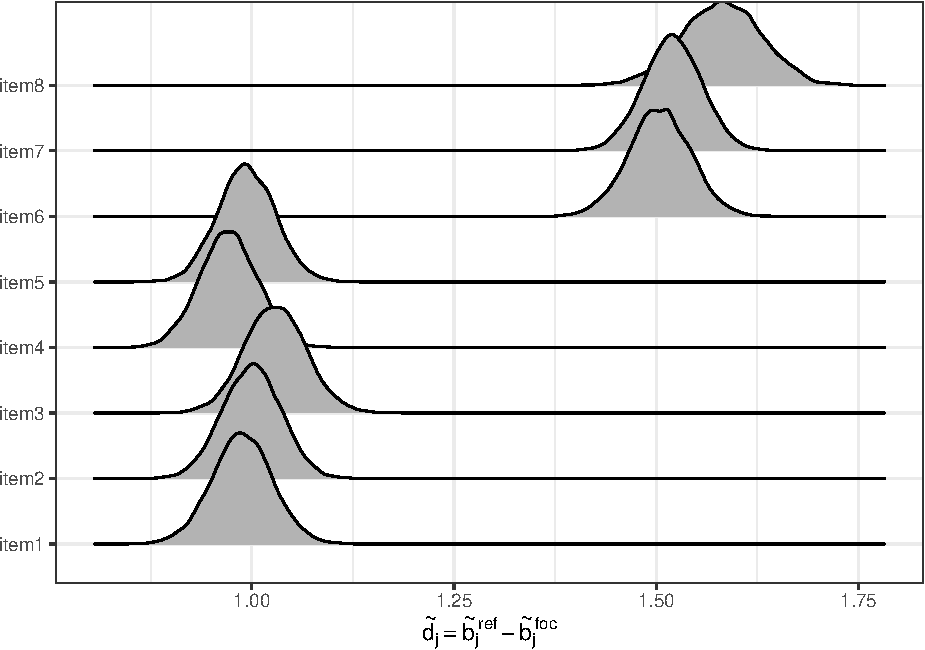
\includegraphics[width=0.7\linewidth]{paper_files/figure-latex/emmilg-1} 

}

\caption{A equal means multiple imputations logit graph (EM-MILG) shows the distribution of how many logits the reference group outperforms the focal group by on each item.}\label{fig:emmilg}
\end{figure}

After choosing the anchor items, the model is refit. The new model is identified by setting \(d_j = 0\) for the anchor items, instead of by setting \(\mu^\text{foc} = 0\). The same process of using multiple imputations to estimate the distribution of \(\tilde{d_j}\) can be used with the new model. Because the equal means assumption is not made, we refer to the resulting visualization as a multiple imputations logit graph (MILG). As expected, in our one-run simulation, selecting the first five items as anchors correctly results in \(\hat d_j \approx 0.5\) for the items with DIF as is shown in the MILG in Figure \ref{fig:milg}.

\begin{figure}[H]

{\centering 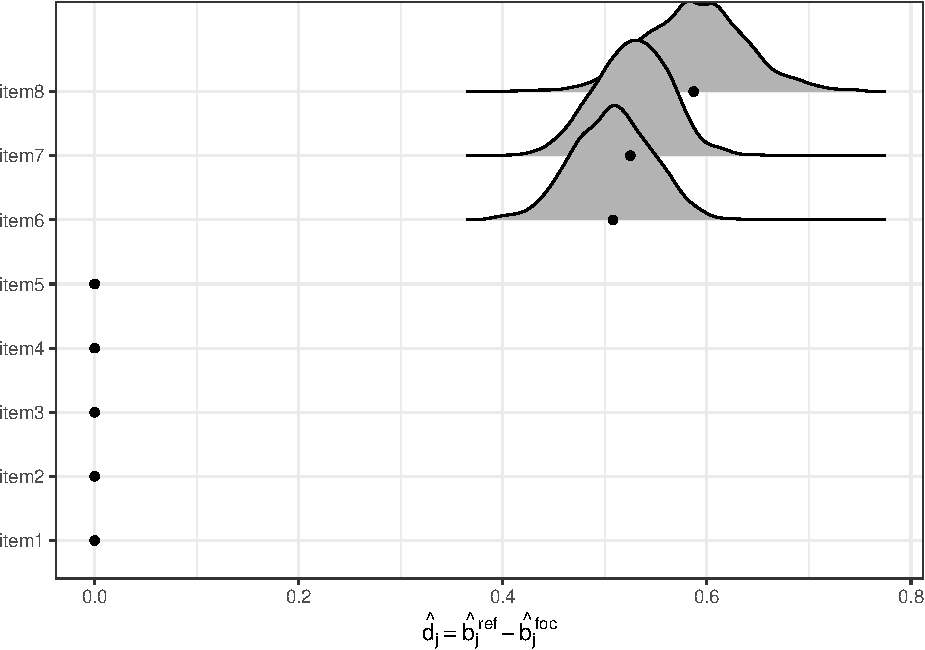
\includegraphics[width=0.7\linewidth]{paper_files/figure-latex/milg-1} 

}

\caption{A multiple imputations logit graph (MILG) shows the distribution of DIF against the focal group. Anchor items are fixed by setting $d_j = 0$.}\label{fig:milg}
\end{figure}

One of our key concerns with typical AI methods is that they can lull the analyst into a false sense of security. Too often, the analyst chooses a method, implements it, and then proceeds as if the method certainly identified the correct anchor items. A EM-MILG combats this concern by presenting all information clearly to the analyst. In the previous example, the analyst may be wary of their results, having seen how arbitrary it was to conclude that the first five and not the last three items are unbiased. Even when other AI methods are used, the analyst can use the EM-MILG as the first step in order to give them a sense of their item response data. And, of course, the MILG can be used to visualize DIF anytime a model is fit using anchor items, not just when the first step involves the EM-MILG. In particular, we could visualize DIF in the non-anchor items after using, for example, AOAA-OAT or EMC to identify the model.

\hypertarget{anchor-points}{%
\subsection{Anchor points}\label{anchor-points}}

The previously discussed AI methods select a set of anchor items, whether it is an algorithm or the analyst that makes that selection. The anchor items are used to estimate \(\hat \mu^\text{foc}\). An alternative strategy is to directly set the anchor point, \(\mu^{\star\text{foc}}\). Anchor point methods have the advantage of not requiring the assumption that any particular item is DIF-free, and, therefore, allowing all items to be tested for DIF. The question then becomes the following: How is the anchor point selected?

\hypertarget{maximizing-the-gini-index-maxgi}{%
\subsubsection{Maximizing the Gini index (MAXGI)}\label{maximizing-the-gini-index-maxgi}}

Strobl et al. (\protect\hyperlink{ref-strobl2018anchor}{2018}) suggest using the Gini index (Gini \protect\hyperlink{ref-gini1912variabilita}{1912}) to select the anchor point. The Gini index is typically used to measure the inequality of wealth distribution in a country. For example, South Africa typically has the highest Gini index of all measured countries, meaning that it is the country with the most unequal wealth distribution (Chitiga, Sekyere, and Tsoanamatsie \protect\hyperlink{ref-chitiga2015income}{2015}). In general, the Gini index \enquote{takes high values if, for example, a small minority of persons has a lot of wealth while the vast majority has very little} (Strobl et al. \protect\hyperlink{ref-strobl2018anchor}{2018}, 7).

\(\mu^{\star\text{foc}}\) is selected by maximizing the Gini index (thus the abbreviation MAXGI). The intuition and assumption is that the items without DIF are the most homogeneous. Denoting a function that calculates the Gini index from a vector of non-negative elements as \(G(\mathbf{x})\), MGI sets
\[
\mu^{\star\text{foc}} = \mathop\mathrm{arg\,max}_{\mu^\text{foc}} G(|\mu^\text{foc} + \tilde{\mathbf{d}}|)
\]
where \(\mu^\text{foc} \in (-\infty, \infty)\) and \(\mu^\text{foc}\) is added to each element of \(\mathbf{d}\).

For our one-run simulation, Figure \ref{fig:ginipath} shows the gini coefficient at a variety of possible \(\mu^\text{foc}\) values. The result of MAXGI is \(\mu^{\star\text{foc}} = -0.99\), which is extraordinarily close to the data-generating value of -1.

\begin{figure}[H]

{\centering 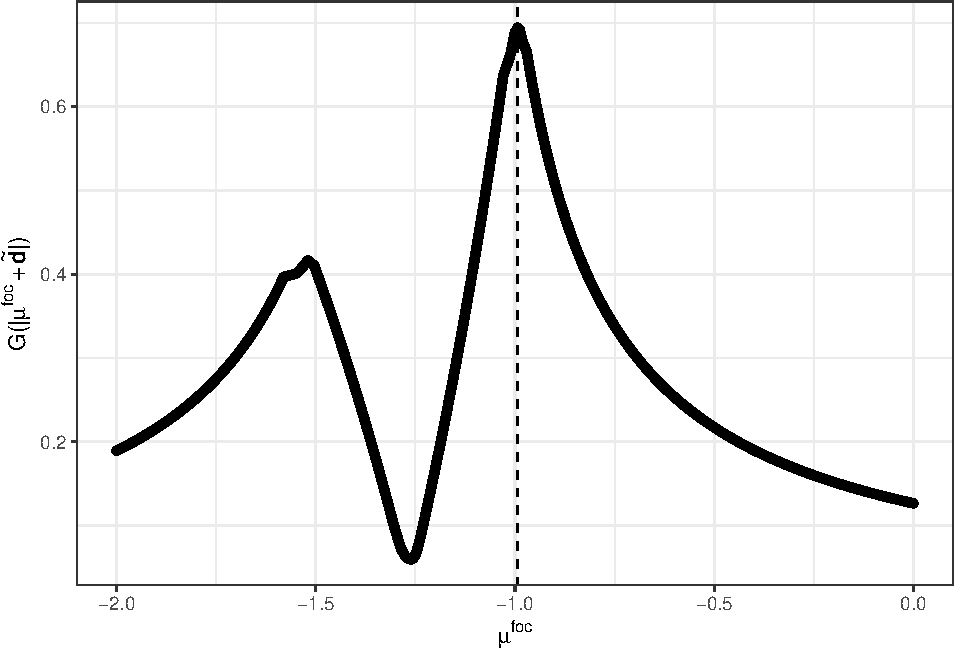
\includegraphics[width=0.7\linewidth]{paper_files/figure-latex/ginipath-1} 

}

\caption{Maximizing the Gini index (MAXGI) to select the anchor point.}\label{fig:ginipath}
\end{figure}

The model is then refit with the identifying assumption that \(\mu^{\text{foc}} = \mu^{\star\text{foc}}\), and the results can be displayed in a MILG as is shown in Figure \ref{fig:ginimilg}.

\begin{figure}[H]

{\centering 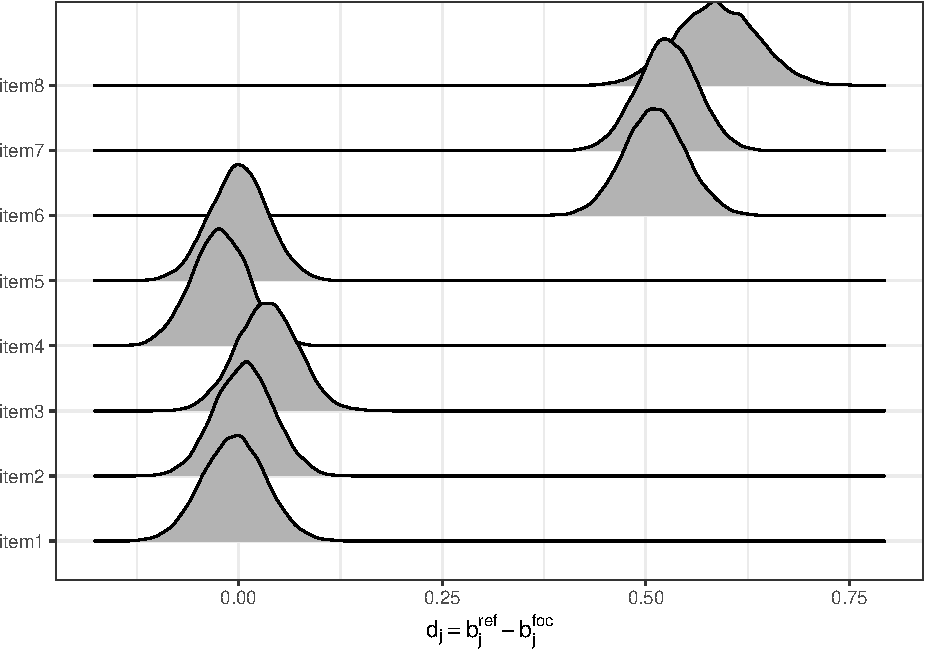
\includegraphics[width=0.7\linewidth]{paper_files/figure-latex/ginimilg-1} 

}

\caption{The MILG with $\mu^{\text{foc}}$ set to $\mu^{\star\text{foc}} = -0.99$.}\label{fig:ginimilg}
\end{figure}

\hypertarget{minimizing-between-curves-minbc}{%
\subsubsection{Minimizing between curves (MINBC)}\label{minimizing-between-curves-minbc}}

Raju's area method (Raju \protect\hyperlink{ref-raju1988area}{1988}) measures the amount of DIF by calculating the area between the item characteristic curves, the function that maps the student's ability to their probability of correct response, of the two groups:
\[
\text{Area Between Curves} = \int |\text{Pr}(y_j = 1| \theta, b_j^{\text{ref}}) - \text{Pr}(y_j = 1| \theta, b_j^{\text{foc}})|
\]
Raju's area method has been cited as one of the most commonly used IRT-based DIF detection methods (Magis et al. \protect\hyperlink{ref-magis2011generalized}{2011}). However, Raju's area method is not an AI method because the item characteristic curves still need to be linked by anchor items or an anchor point. An additional weakness is that the area is unweighted, so all values of \(\theta\) matter equally, despite some being much more realistic than others.

To adapt Raju's area method into an AI method, we propose a new method, which we call \enquote{minimizing the area between curves} (MINBC). To understand MINBC, imagine a scenario in which the data-generating process is \(\mu^{\text{foc}} = \mu^{\text{ref}}\) and \(d_j = 0 \forall j\), so that there is no DIF. The fundamental identification problem is that there are an infinite number of models with the same likelihood from which to choose. For example, we could correctly assume that the focal group has the same ability as the reference group and fix \(\mu^{\star\text{foc}} = 0\). The model would then estimate \(\hat d_j \approx 0 \forall j\), and we would correctly conclude the groups have the same ability and there is no DIF. Alternatively, we could assume that the focal group has \(\mu^{\star\text{foc}} = 3\). The model would then compensate by finding \(\hat d_j \approx -3 \forall j\), and we would incorrectly conclude that the focal group is high ability, but every item contains DIF against them. Both of these models have the same likelihood, so how should one choose which model to believe? MINBC chooses the model with the least amount of total DIF, as measured by the total weighted area between the item characteristic curves. As a result, the likelihood tie is broken by preferring to explain differences in performance across groups by ability differences (as opposed to DIF).

Denote a function that takes \(\mu^\text{foc}\) as input and estimates \(\hat b_j^\text{foc}\) by fitting a unidimensional Rasch model as \(m_j(\mu^\text{foc})\). The amount of DIF on each item is calculated as
\[
\text{DIF}_j(\mu^\text{foc}) = \int |\text{Pr}(y_j = 1| \theta, b_j^{\text{ref}}) - \text{Pr}(y_j = 1| \theta, m_j(\mu^\text{foc}))| g(\theta)d\theta
\]
where \(g(\theta)\) is a weighting function such that \(\int g(\theta)d\theta = 1\). The total DIF on the test, then, is
\[
\text{Total DIF}(\mu^\text{foc}) = \sum_{j} \text{DIF}_j(\mu^\text{foc})
\]
In this way, \(\text{Total DIF}(\mu^\text{foc})\) is a function where the input is \(\mu^\text{foc}\) and the output is the total amount of DIF on the test. MINBC sets
\[
\mu^{\star\text{foc}} = \mathop\mathrm{arg\,min}_{\mu^\text{foc}} \text{Total DIF}(\mu^\text{foc}).
\]
MINBC is inspired in part by Chalmers, Counsell, and Flora (\protect\hyperlink{ref-chalmers2016might}{2016}), who use the difference between test characteristic curves weighted by \(g(\theta)\) as a measure of differential test functioning (DTF). The selection of \(g(\theta)\) results in the relative weighting of \(\theta\) values. Chalmers, Counsell, and Flora do not discuss how to choose \(g(\theta)\) and in their empirical examples use \(g(\theta)\) uniform for \(-6 \le \theta \le 6\), which may be suboptimal in some cases. It might seem intuitive to choose \(g(\theta) \sim N(0, 1)\) because \(\mu^\text{ref} = 0\), but this choice doesn't take into account the ability distribution of the focal group. If \(\mu^\text{foc} = 3\), wouldn't we also want to prioritize high \(\theta\) values? Accordingly, we set \(g(\theta)\) to be the average of the reference and focal group ability probability density functions:
\[
g(\theta) = \dfrac{N(\mu^{\text{ref}}, \sigma^{\text{ref}^2}) + N(\mu^{\text{foc}}, \sigma^{\text{foc}^2})}{2}.
\]

For our one-run simulation, Figure \ref{fig:mabc} shows Total DIF at a variety of possible values for \(\mu^\text{foc}\). In this case, MINBC works perfectly and the anchor point is found to be \(\mu^{\star\text{foc}} = -1\). As with MAXGI, the model should then be refit using the identifying assumption that \(\mu^{\text{foc}} = \mu^{\star\text{foc}}\).

\begin{figure}[H]

{\centering 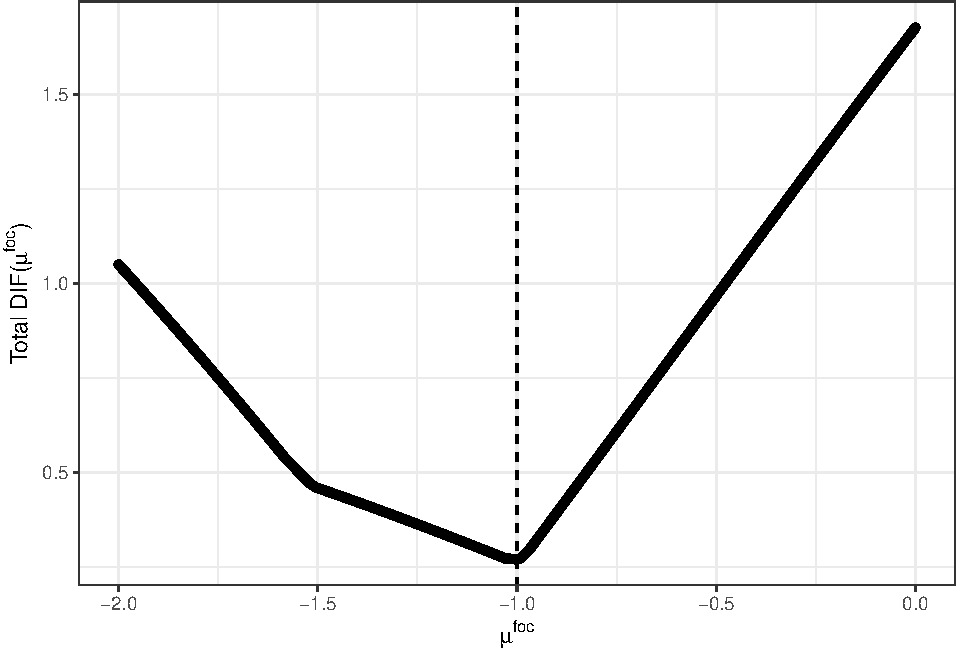
\includegraphics[width=0.7\linewidth]{paper_files/figure-latex/mabc-1} 

}

\caption{Minimizing the area between curves (MINBC) to select the anchor point.}\label{fig:mabc}
\end{figure}

\hypertarget{summary-of-ai-methods}{%
\subsection{Summary of AI methods}\label{summary-of-ai-methods}}

We have described a variety of AI methods and their corresponding acronymns. Some of these methods, such as AOAA and EMC, select anchor items, while others, such as MAXGI and MINBC, select an anchor point. Table \ref{table:allmethods} summarizes all of these methods.

\begin{table}[H]
\caption{Summary of agnostic identification methods}
\centering
\begin{tabular}{|p{4cm}|p{6cm}|p{4cm}|}
\toprule

Method & Description & Literature \\

\midrule

all-others-as-anchors (AOAA) & See Table \ref{table:themethods} for a summary of all three AOAA methods. &  \\\hline

equal means clustering (EMC) & Cluster items based on differences in performance across groups and choose one of the clusters to be the anchor cluster. & Proposed by \cite{bechger2015statistical} and refined by \cite{pohl2017cluster} \\\hline

equal means, multiple imputation logit graph (EM-MILG) & Arbitrarily set both group means to 0, which pushes all group performance differences to the item paramaters, measure variability using multiple imputations, and graph the result. Can be used by an analyst to hand select anchor items & Inspired by pedagolical examples \cite{pohl2017cluster} and \cite{talbot2013taking} \\\hline

multiple imputation logit graph (MILG) & Similar to EM-MILG but used to visualize potential DIF once the model is already identified &  \\\hline

maximizing Gini index (MAXGI) & Arbitrarily set both group means to 0 and then choose an anchor point by maximizing the Gini index & Adapted from work by \cite{strobl2018anchor} \\\hline

minimizing the area between curves (MINBC) & Of the infinite number of model that maximizes the likelihood of the data, choose the one with the minimum total area between the two groups' item characteristic curves & Built on and inspired by work by \cite{raju1988area} and more recently, \cite{chalmers2016might} \\

\bottomrule
\end{tabular}
\label{table:allmethods}
\end{table}

\hypertarget{simulation-study}{%
\section{Simulation study}\label{simulation-study}}

To compare each of the methods in Table \ref{table:allmethods}, we conducted a simulated study. Our goal was to make the data generating process as realistic to the scenario described by Ackerman (\protect\hyperlink{ref-ackerman1992didactic}{1992}) in which some items on a math test also depend on a student's verbal ability (the target ability is math ability, and the nuisance ability is verbal ability). As described in \protect\hyperlink{intro}{the introduction}, nearly all DIF simulation studies in the literature generate data by simply altering the item easiness parameters for the focal group. This setup can be re-written as a two-dimensional compensatory item response model where nuisance ability is the same for all students from the same group. One exception is Walker and Gocer Sahin (\protect\hyperlink{ref-walker2017using}{2017}) who draw each student's target ability and nuisance ability from a two-dimensional normal distribution with varying covariance matrices.

In our simulation study, it was critical that student ability was drawn in a realistic way similar to Walker and Gocer Sahin (\protect\hyperlink{ref-walker2017using}{2017}). However, we don't believe that a compensatory model is realistic in describing a math test where some items depend on verbal ability. For example, it's hard to imagine that a student without the verbal ability to parse a word problem could fully compensate by having a higher math ability. Accordingly, we generate item responses using a simplified version of Sympson's (\protect\hyperlink{ref-sympson1978model}{1978}) noncompensatory item response model in which
\[
\text{Pr}(y_{ij} = 1 | \theta_i, \eta_i, a_{2j}) = \sigma(\theta_i) \cdot \sigma(a_{2j}\eta_i)
\]
where, as before, \(\theta_i\) is target ability, \(\eta_i\) is nuisance ability, and \(\sigma(a_{2j})\) is the item's loading on nuisance ability (DeMars \protect\hyperlink{ref-demars2016partially}{2016}).

\hypertarget{drawing-parameters}{%
\subsection{Drawing parameters}\label{drawing-parameters}}

In each run, we simulate 10,000 students with half coming from each of the reference and focal groups. For students from the reference group, target ability and nuisance ability are drawn from the two-dimensional normal distribution with mean {[}\(\mu_\theta^\text{ref} = 0\), \(\mu_\eta^\text{ref} = 0\){]} and covariance matrix \(\begin{bmatrix} 1 & 0.5 \\ 0.5 & 1 \end{bmatrix}\). Abilities for students from the focal group are drawn using the same covariance matrix, but with means {[}\(\mu_\theta^\text{foc} = -0.5\), \(\mu_\eta^\text{foc} = -1\){]}.

The test always has 12 items, but we vary the number of items with DIF from two to six. For items without DIF, \(a_{2j} = \infty\) so that the model reduces to \(\text{Pr}(y_{ij} = 1 | \theta_i) = \sigma(\theta_i)\). For items with DIF, \(a_{2j}\) is calculated based on Ackerman's (\protect\hyperlink{ref-ackerman1994using}{1994}) angle equation as described in Walker and Gocer Sahin (\protect\hyperlink{ref-walker2017using}{2017}):
\[
\angle_j = \arccos \dfrac{a_{1j}^2}{a_{1j}^2 + a_{2j}^2}.
\]
An item's angle measures the relative loading of the item on the two dimensions. For example, an angle of 45\(^\circ\) indicates that the item loads equally on the target ability and nuisance ability. Our simple noncompensatory model has \(a_{1j} = 1\) for all items so the angle equation reduces to
\[
\angle_j = \arccos \dfrac{1}{1 + a_{2j}^2}.
\]
We are interested in specifying the angle of an item, so the relevant equation becomes
\[
a_{2j} = \sqrt{\dfrac{1 - \cos(\angle_j)^2}{\cos(\angle_j)^2}}.
\]
For DIF items, we set \(a_{2j}\) based on angles with equal intervals between 20\(^\circ\) and 60\(^\circ\). For example, for a test with three DIF items the angles are 20\(^\circ\), 40\(^\circ\), and 60\(^\circ\).

\hypertarget{visualizing-a-run}{%
\subsection{Visualizing a run}\label{visualizing-a-run}}

Figure \ref{fig:difmap} provides intuition about the data generating process by showing the relationship between \(\theta_i\) and \(Pr(y_{ij} = 1)\) with \(\eta_i\) set to the group mean for a test with six DIF items. The items are ordered by the amount of DIF such that \(\angle_{j = 7} = 20^\circ\) up to \(\angle_{j = 12} = 60^\circ\).

\begin{figure}[H]

{\centering 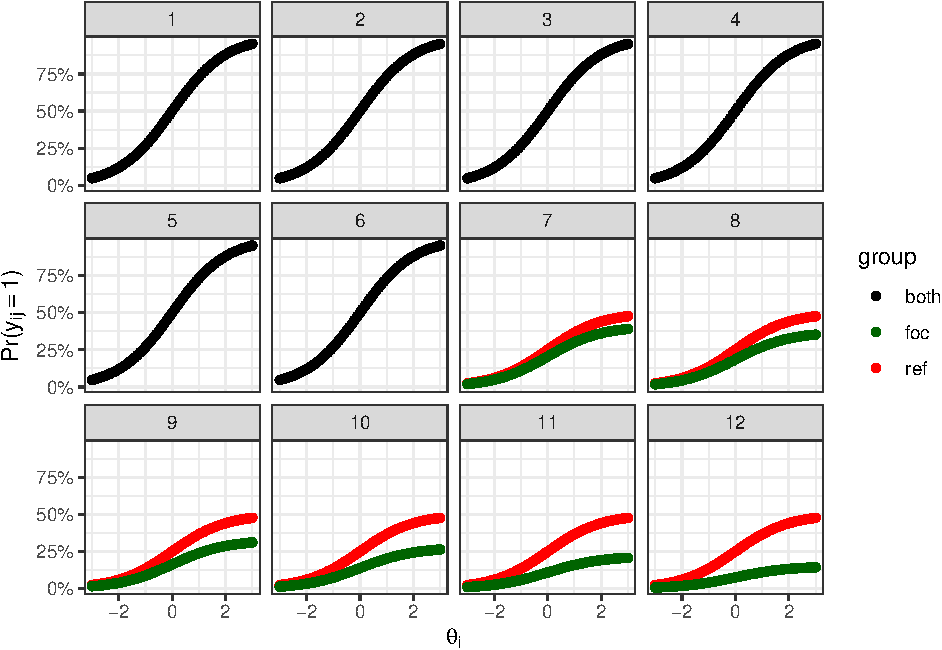
\includegraphics[width=0.7\linewidth]{paper_files/figure-latex/difmap-1} 

}

\caption{For a 12 item test containing 6 items with DIF, the relationship between target ability and probability of correct response with nuisance abilities fixed to the group mean.}\label{fig:difmap}
\end{figure}

Figure \ref{fig:simemmlg} shows the EM-MILG --- generated using a Rasch model where both group means are fixed to 0 and item parameters are estimated freely as described in the \protect\hyperlink{anchoritems}{the anchor items section} --- for one run using the same item parameters that generated Figure \ref{fig:difmap}. As expected, \(\tilde{d_j}\) is about \(\mu_\theta^\text{foc} - \mu_\theta^\text{ref} = -0.5 - 0 = -0.5\) for the first six items which are DIF free. For the last six items, \(\tilde{d_j}\) increases as \(\angle_j\) increases.

\begin{figure}[H]

{\centering 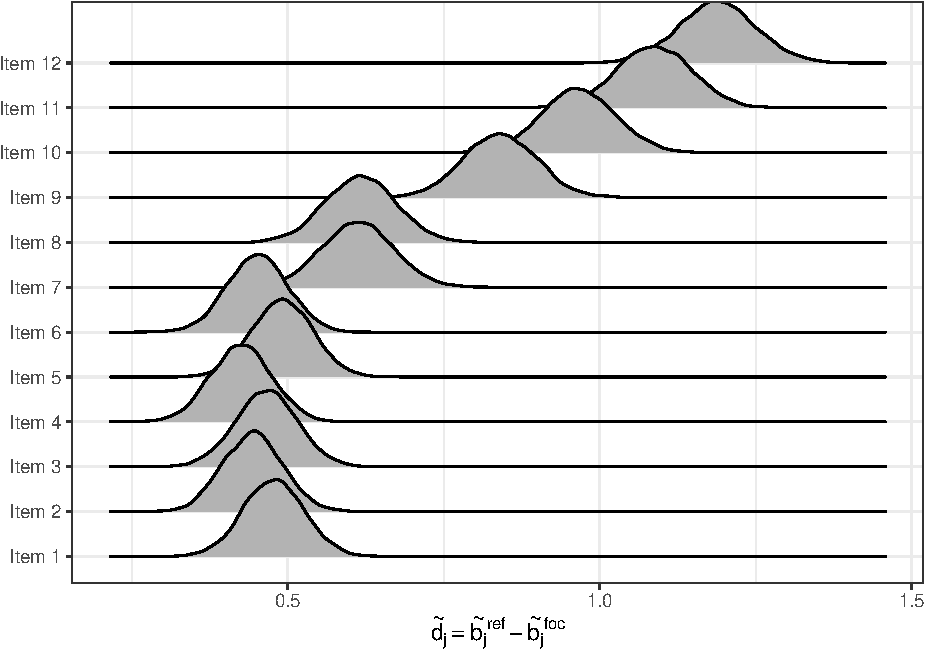
\includegraphics[width=0.7\linewidth]{paper_files/figure-latex/simemmlg-1} 

}

\caption{For a 20 item test, the relationship between target ability and probability of correct response with nuisance abilities fixed to group means.}\label{fig:simemmlg}
\end{figure}

\hypertarget{outcomes}{%
\subsection{Outcomes}\label{outcomes}}

For each run, we applied each AI method to find the method's identifying assumption. The method's identifying assumption was then used to fit a final model. We compared the performance of those final models according to the following outcomes.

\hypertarget{achievement-gap-residual}{%
\subsubsection{Achievement gap residual}\label{achievement-gap-residual}}

An effective AI method should lead to a final model that accurately estimates the difference between the reference group's mean target ability and the focal group's mean target ability. We refer to this quantity as the achievement gap. Recall that all models set \(\mu_\theta^\text{ref} = 0\), so the achievement gap reduces to \(\mu_\theta^\text{ref}\). The data-generating value of \(\mu_\theta^\text{foc}\) is 0.5, but each run will include sampling variability. To get at the heart of how well a method is doing, we calculated the achievement gap residual as the method's estimated achievement gap, \(\hat\mu_\theta^\text{foc}\), minus the achievement gap estimated when using only the DIF-free items as anchors. In summary, this outcome measures a method's ability to disentangle differences in target ability from nuisance ability at the group level.

\hypertarget{individual-abilities}{%
\subsubsection{Individual abilities}\label{individual-abilities}}

Assessments are frequently used to make decisions about individual student abilities. We measured a method's ability to do so by calculating the rank correlation between the vector of estimated abilities and the vector of true target abilities. We used rank correlation as opposed to the more typically used RMSE in agreement with Lord's (\protect\hyperlink{ref-lord1986maximum}{1986}) argument that RMSE can be inflated by poor performance at the extremes of ability for which the test was not designed to measure precisely. \emph{(TODO: this isn't included in this current draft, and I'm not actually sure it's necessary. maybe this idea of rank order being better than RMSE is for another paper)}

\hypertarget{anchor-items.}{%
\subsubsection{Anchor items.}\label{anchor-items.}}

For the methods that choose a set of anchor items, we looked directly at which anchor items were selected. An effective method should use most of the non-DIF items as anchors (the anchor hit rate) while avoiding using items with DIF as anchors (the false anchor rate).

\hypertarget{results}{%
\subsection{Results}\label{results}}

In total, we executed 100 runs for each of two, three, four, five, and six DIF items. Figure \ref{fig:achievegap} shows each method's performance on the achievement gap residual. AOAA-OAT is the clear winner. It performed nearly perfectly for two, three, or four DIF items. Even when six of the 12 items on the test contained DIF, AOAA-OAT underestimated \(\mu_\theta^\text{foc}\) by only 0.05 standard deviations on its worst run. As expected, artificial DIF caused AOAA and AOAA-AS to go off the rails as the number of DIF items increases.

EMC performed better than AOAA and AOAA-AS, but worse than the other methods. MINBC and MAXGI performed similarly well with MINBC estimating the achievement gap with more precision but more bias than MAXGI, especially for tests with more than four DIF items. We hypothesize that MINBC's susceptibility to bias results from considering every item, including the items with DIF, whereas as soon as, for example, AOAA-OAT, removes an item from the anchor set, it is thereafter completely disregarded by the method.

\begin{figure}[H]

{\centering 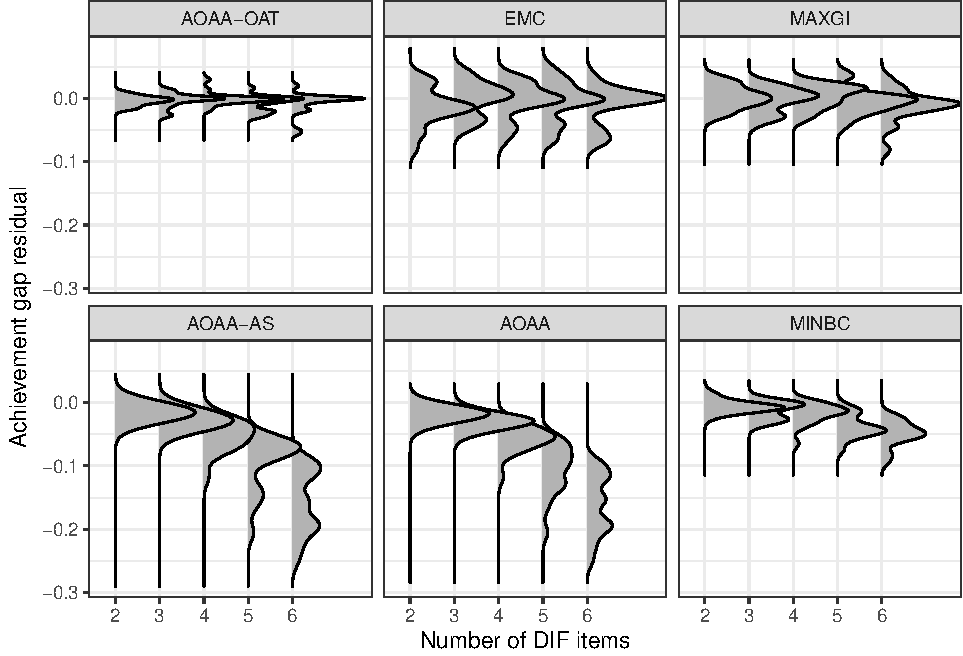
\includegraphics[width=0.7\linewidth]{paper_files/figure-latex/achievegap-1} 

}

\caption{Achievement gap residual distributions across 100 runs for each AI method and number of DIF items.}\label{fig:achievegap}
\end{figure}

Figure \ref{fig:anchorfalse} shows the mean false anchor rates for each method and number of items with DIF. For example, when there were two items with DIF on the test, those two items had \(\angle_{11} = 20^\circ\) and \(\angle_{12} = 60^\circ\). AOAA-OAT never included item 12 in the anchor set, but incorrectly included item 11 in 60 out of the 100 runs. Accordingly, the mean false anchor rate for two DIF items and the AOAA-OAT method was
\[
\dfrac{\text{Total number of DIF items in the anchor set}}{\text{Number of DIF items on each test} \cdot \text{Number of runs}} = \dfrac{60}{2 \cdot 100} = 30\%.
\]
The fact that the item with 20\(^\circ\) of DIF is most commonly incorrectly included in the anchor set is what drove the counterintuitive result that the mean false anchor rate decreases with more DIF items.

Similarly, Figure \ref{fig:anchorhit} shows the mean anchor hit rates. Remarkably, AOAA-OAT included an average of over \(90\%\) of DIF-free items in the anchor set regardless of the number of DIF items on the test. Interestingly, EMC had a better anchor hit rate on tests with more DIF items. This result appears to be driven by the clustering algorithm sometimes splitting all of the DIF-free items into two separate clusters, especially when most of the items are DIF-free.

\begin{figure}[H]

{\centering 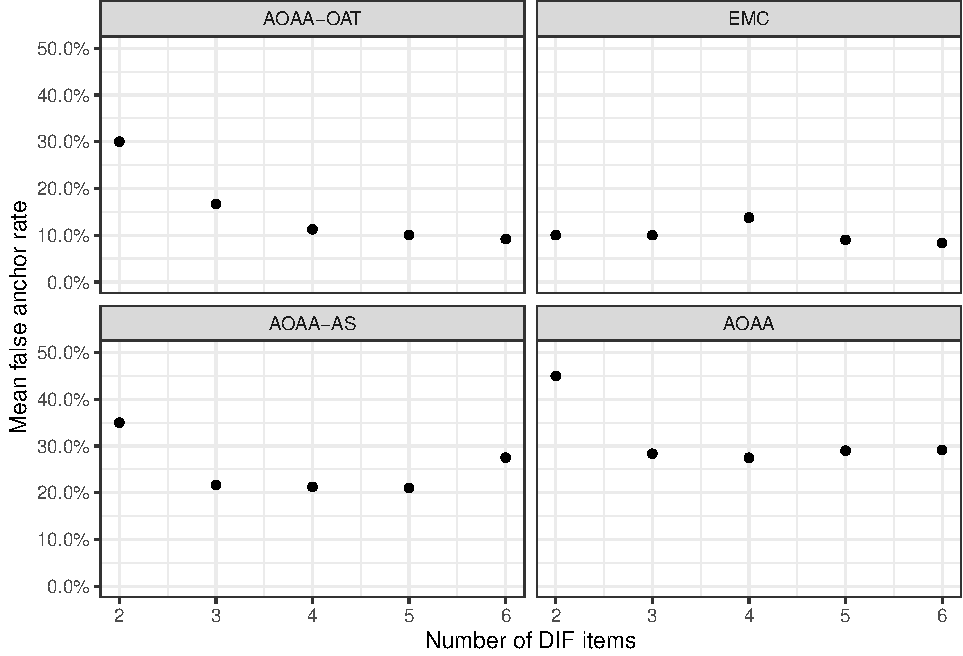
\includegraphics[width=0.7\linewidth]{paper_files/figure-latex/anchorfalse-1} 

}

\caption{Mean false anchor rates across 100 runs for each AI method and number of DIF items.}\label{fig:anchorfalse}
\end{figure}

\begin{figure}[H]

{\centering 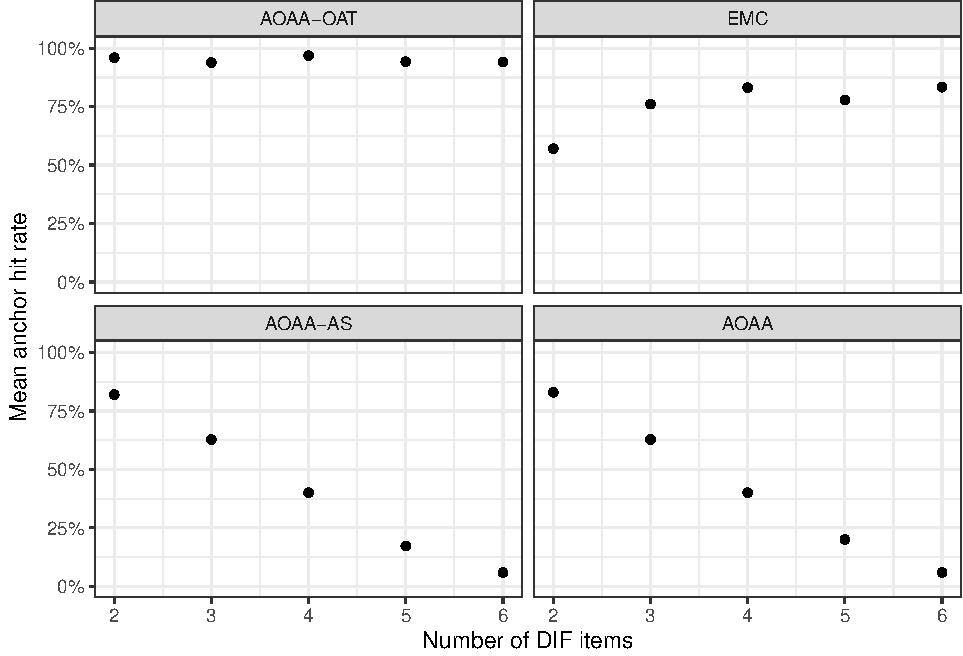
\includegraphics[width=0.7\linewidth]{paper_files/figure-latex/anchorhit-1} 

}

\caption{Mean anchor hit rates across 100 runs for each AI method and number of DIF items.}\label{fig:anchorhit}
\end{figure}

\hypertarget{discussion-and-summary}{%
\section{Discussion and summary}\label{discussion-and-summary}}

Measurement instruments need to be inspected for DIF so that we can be sure of the validity of the conclusions that we draw regardless of the group membership of each student. Inspired by Ackerman (\protect\hyperlink{ref-ackerman1992didactic}{1992}), we have resurrected the DIF-as-student-property view and shown its connection to the typical way in which AI methods and DIF simulation studies have been conceptualized.

More importantly, we reviewed a variety of AI methods, proposed new AI methods, and tested their performance in a simulation study that we believe to be more realistic than the typical DIF simulation study. In particular, we simulated student ability as drawn from a two-dimensional distribution representing a student's target and nuisance ability, and then generated data using a noncompensatory item response model. Our simulation results showed that two of the most common AI methods, AOAA and AOAA-AS, perform quite poorly, especially as the number of items containing DIF grows. On the other hand, AOAA-OAT, EMC, MINGI, and MAXBC all performed reasonably.

In particular, AOAA-OAT was the clear winner, and we recommend its use whenever possible. One reason AOAA-OAT might not always be possible is that it can be computationally expensive. For example, finding three items containing DIF on a 12-item test requires fitting 46 item response models, and that number grows as either the test length or the number of items testing positive for DIF grows. To increase AOAA-OAT's use, we recommend its implementation (perhaps as the default) in popular IRT software such as the mirt R package.

In addition to exploring and testing algorithmic AI methods, we introduced a method, the EM-MILG, that an analyst can use to visualize the amount of potential DIF in their data. This method can be used either to build their intuition or as a way in which they can select anchor items by hand. The EM-MILG's sibling method, the MILG, is, we believe, the best way to visualize the results of a DIF analysis after anchor items have been selected.

Future work should test these methods' performance under a greater variety of data-generating conditions. For example, changing the compensatory nature of the data generating model or adding additional nuisance ability dimensions. Furthermore, our work focused on the Rasch model, and it will be of great interest to consider how these methods extend and perform when the goal is to detect and correct for DIF when fitting a 2PL or 3PL item response model.

\clearpage

\bibliographystyle{apa}
\bibliography{paper.bib}

\hypertarget{refs}{}
\leavevmode\hypertarget{ref-ackerman1992didactic}{}%
Ackerman, Terry A. 1992. ``A Didactic Explanation of Item Bias, Item Impact, and Item Validity from a Multidimensional Perspective.'' \emph{Journal of Educational Measurement} 29 (1): 67--91.

\leavevmode\hypertarget{ref-ackerman1994using}{}%
---------. 1994. ``Using Multidimensional Item Response Theory to Understand What Items and Tests Are Measuring.'' \emph{Applied Measurement in Education} 7 (4): 255--78.

\leavevmode\hypertarget{ref-andrich2012real}{}%
Andrich, David, and Curt Hagquist. 2012. ``Real and Artificial Differential Item Functioning.'' \emph{Journal of Educational and Behavioral Statistics} 37 (3): 387--416.

\leavevmode\hypertarget{ref-bechger2015statistical}{}%
Bechger, Timo M, and Gunter Maris. 2015. ``A Statistical Test for Differential Item Pair Functioning.'' \emph{Psychometrika} 80 (2): 317--40.

\leavevmode\hypertarget{ref-camilli1992conceptual}{}%
Camilli, Gregory. 1992. ``A Conceptual Analysis of Differential Item Functioning in Terms of a Multidimensional Item Response Model.'' \emph{Applied Psychological Measurement} 16 (2): 129--47.

\leavevmode\hypertarget{ref-chalmers2012mirt}{}%
Chalmers, R Philip. 2012. ``Mirt: A Multidimensional Item Response Theory Package for the R Environment.'' \emph{Journal of Statistical Software} 48 (6): 1--29.

\leavevmode\hypertarget{ref-chalmers2018numerical}{}%
---------. 2018. ``Numerical Approximation of the Observed Information Matrix with Oakes' Identity.'' \emph{British Journal of Mathematical and Statistical Psychology} 71 (3): 415--36.

\leavevmode\hypertarget{ref-chalmers2016might}{}%
Chalmers, R Philip, Alyssa Counsell, and David B Flora. 2016. ``It Might Not Make a Big Dif: Improved Differential Test Functioning Statistics That Account for Sampling Variability.'' \emph{Educational and Psychological Measurement} 76 (1): 114--40.

\leavevmode\hypertarget{ref-chitiga2015income}{}%
Chitiga, Margaret, E Sekyere, and N Tsoanamatsie. 2015. ``Income Inequality and Limitations of the Gini Index: The Case of South Africa.'' \emph{Human Sciences Research Council (HSRC), Available at: Http://Www. Hsrc. Ac. Za/En/Review/Hsrc-Review-November-2014/Limitations-of-Gini-Index, Site Accessed} 2.

\leavevmode\hypertarget{ref-demars2016partially}{}%
DeMars, Christine E. 2016. ``Partially Compensatory Multidimensional Item Response Theory Models: Two Alternate Model Forms.'' \emph{Educational and Psychological Measurement} 76 (2): 231--57.

\leavevmode\hypertarget{ref-drasgow1987study}{}%
Drasgow, Fritz. 1987. ``Study of the Measurement Bias of Two Standardized Psychological Tests.'' \emph{Journal of Applied Psychology} 72 (1): 19.

\leavevmode\hypertarget{ref-edelen2006identification}{}%
Edelen, Maria Orlando, David Thissen, Jeanne A Teresi, Marjorie Kleinman, and Katja Ocepek-Welikson. 2006. ``Identification of Differential Item Functioning Using Item Response Theory and the Likelihood-Based Model Comparison Approach: Application to the Mini-Mental State Examination.'' \emph{Medical Care}, S134--S142.

\leavevmode\hypertarget{ref-gini1912variabilita}{}%
Gini, Corrado. 1912. ``Variabilità E Mutabilità (Variability and Mutability).'' \emph{Tipografia Di Paolo Cuppini, Bologna, Italy}, 156.

\leavevmode\hypertarget{ref-hagquist2017recent}{}%
Hagquist, Curt, and David Andrich. 2017. ``Recent Advances in Analysis of Differential Item Functioning in Health Research Using the Rasch Model.'' \emph{Health and Quality of Life Outcomes} 15 (1): 181.

\leavevmode\hypertarget{ref-hastie2001estimating}{}%
Hastie, Trevor, Robert Tibshirani, and Guenther Walther. 2001. ``Estimating the Number of Data Clusters via the Gap Statistic.'' \emph{J Roy Stat Soc B} 63: 411--23.

\leavevmode\hypertarget{ref-holland1986differential}{}%
Holland, Paul W, and Dorothy T Thayer. 1986. ``Differential Item Functioning and the Mantel-Haenszel Procedure.'' \emph{ETS Research Report Series} 1986 (2): i--24.

\leavevmode\hypertarget{ref-kopf2015framework}{}%
Kopf, Julia, Achim Zeileis, and Carolin Strobl. 2015. ``A Framework for Anchor Methods and an Iterative Forward Approach for Dif Detection.'' \emph{Applied Psychological Measurement} 39 (2): 83--103.

\leavevmode\hypertarget{ref-lord1986maximum}{}%
Lord, Frederic M. 1986. ``Maximum Likelihood and Bayesian Parameter Estimation in Item Response Theory.'' \emph{Journal of Educational Measurement} 23 (2): 157--62.

\leavevmode\hypertarget{ref-magis2011generalized}{}%
Magis, David, Gilles Raı̂che, Sébastien Béland, and Paul Gérard. 2011. ``A Generalized Logistic Regression Procedure to Detect Differential Item Functioning Among Multiple Groups.'' \emph{International Journal of Testing} 11 (4): 365--86.

\leavevmode\hypertarget{ref-meade2012solving}{}%
Meade, Adam W, and Natalie A Wright. 2012. ``Solving the Measurement Invariance Anchor Item Problem in Item Response Theory.'' \emph{Journal of Applied Psychology} 97 (5): 1016.

\leavevmode\hypertarget{ref-pohl2017cluster}{}%
Pohl, Steffi, Eric Stets, and Claus H Carstensen. 2017. ``Cluster-Based Anchor Item Identification and Selection.''

\leavevmode\hypertarget{ref-raju1988area}{}%
Raju, Nambury S. 1988. ``The Area Between Two Item Characteristic Curves.'' \emph{Psychometrika} 53 (4): 495--502.

\leavevmode\hypertarget{ref-rcore}{}%
R Core Team. 2019. \emph{R: A Language and Environment for Statistical Computing}. Vienna, Austria: R Foundation for Statistical Computing. \url{https://www.R-project.org/}.

\leavevmode\hypertarget{ref-stark2006detecting}{}%
Stark, Stephen, Oleksandr S Chernyshenko, and Fritz Drasgow. 2006. ``Detecting Differential Item Functioning with Confirmatory Factor Analysis and Item Response Theory: Toward a Unified Strategy.'' \emph{Journal of Applied Psychology} 91 (6): 1292.

\leavevmode\hypertarget{ref-strobl2018anchor}{}%
Strobl, Carolin, Julia Kopf, Raphael Hartmann, and Achim Zeileis. 2018. ``Anchor Point Selection: An Approach for Anchoring Without Anchor Items.'' Working Papers in Economics; Statistics.

\leavevmode\hypertarget{ref-swaminathan1990detecting}{}%
Swaminathan, Hariharan, and H Jane Rogers. 1990. ``Detecting Differential Item Functioning Using Logistic Regression Procedures.'' \emph{Journal of Educational Measurement} 27 (4): 361--70.

\leavevmode\hypertarget{ref-sympson1978model}{}%
Sympson, James B. 1978. ``A Model for Testing with Multidimensional Items.'' In \emph{Proceedings of the 1977 Computerized Adaptive Testing Conference}. 00014.

\leavevmode\hypertarget{ref-talbot2013taking}{}%
Talbot III, Robert M. 2013. ``Taking an Item-Level Approach to Measuring Change with the Force and Motion Conceptual Evaluation: An Application of Item Response Theory.'' \emph{School Science and Mathematics} 113 (7): 356--65.

\leavevmode\hypertarget{ref-thissen1993detection}{}%
Thissen, David, Lynne Steinberg, and Howard Wainer. 1993. ``Detection of Differential Item Functioning Using the Parameters of Item Response Models.''

\leavevmode\hypertarget{ref-walker2017using}{}%
Walker, Cindy M, and Sakine Gocer Sahin. 2017. ``Using a Multidimensional Irt Framework to Better Understand Differential Item Functioning (Dif): A Tale of Three Dif Detection Procedures.'' \emph{Educational and Psychological Measurement} 77 (6): 945--70.

\leavevmode\hypertarget{ref-tidy}{}%
Wickham, Hadley. 2017. \emph{Tidyverse: Easily Install and Load the 'Tidyverse'}. \url{https://CRAN.R-project.org/package=tidyverse}.

\leavevmode\hypertarget{ref-woods2009empirical}{}%
Woods, Carol M. 2009. ``Empirical Selection of Anchors for Tests of Differential Item Functioning.'' \emph{Applied Psychological Measurement} 33 (1): 42--57.

\leavevmode\hypertarget{ref-yang2012characterizing}{}%
Yang, Ji Seung, Mark Hansen, and Li Cai. 2012. ``Characterizing Sources of Uncertainty in Item Response Theory Scale Scores.'' \emph{Educational and Psychological Measurement} 72 (2): 264--90.

\end{document}
